\documentclass[aspectratio=169]{beamer}
\usepackage[english]{babel}
\usepackage[utf8]{inputenc}

% AMSLaTeX packages
\usepackage{amsthm}
\usepackage{amsmath}
\usepackage{amsfonts}
\usepackage[algoruled]{algorithm2e}

\usetheme{default}
\useoutertheme{default}
% we want to use images
\usepackage{graphicx}
\usepackage{movie15}
\usepackage{hyperref}

% table relates packages
\usepackage{booktabs}
\usepackage{multirow}
% pick a font
\usepackage{palatino}           
% \usepackage{times}
\usepackage{tikz}
\usetikzlibrary[positioning,arrows,decorations.pathmorphing,backgrounds,fit,calc]
% \AtBeginSection[]  % "Beamer, do the following at the start of every section"
% {
%   \begin{frame}<beamer> 
%     \frametitle{Outline} % make a frame titled "Outline"
%     \tableofcontents[currentsection]  % show TOC and highlight current section
%   \end{frame}                    
% }

% \AtBeginSubsection[]
% {
%   \begin{frame}
%     \frametitle{Outline}
%     \tableofcontents[currentsection,currentsubsection]
%   \end{frame}
% }

\AtBeginSection[]
{
   \begin{frame}
       \frametitle{Outline}
       \tableofcontents[currentsection]
   \end{frame}
}

\newcommand{\ebox}[1][1em]{\framebox[#1]{\phantom{M}}}

\setlength\arraycolsep{1.4pt}% some length

%gets rid of navigation symbols
\setbeamertemplate{navigation symbols}{}

%gets rid of bottom navigation bars
\setbeamertemplate{footline}[page number]{}
\setbeamertemplate{headline}{}



% Get cmark and xmark
\usepackage{pifont}
\newcommand{\cmark}{\ding{51}}
\newcommand{\xmark}{\ding{55}}

\usebackgroundtemplate{
\includegraphics[width=\paperwidth]{NormalANLBlue}}

\title[]{\bigskip\\
	Multiobjective Optimization of the Variability of the High-Performance
	LINPACK Solver}
\author[]{\vskip -20pt
	Tyler Chang$^{a,b}$, Jeffrey Larson$^b$, and Layne Watson$^a$}
\institute[]{$^a$Dept. of Computer Science, Virginia Tech\\ \medskip
$^b$Mathematics and Computer Science Division, Argonne National Laboratory}
\date{December 18, 2020}

\begin{document}

\setbeamertemplate{footline}{}
{
\usebackgroundtemplate{
\includegraphics[width=\paperwidth]{TitleANLBlue}}
\frame{\titlepage}
}

\setbeamertemplate{footline}[page number]{}

% FRAME: overview
\begin{frame}
  \frametitle{Outline}
  \tableofcontents
\end{frame}

% ========================================
% main slides come here
% ========================================
\section{Introduction and Motivation}

\begin{frame}\frametitle{Performance Variability}
	\begin{columns}
	\begin{column}{0.5\textwidth}
		\textbf{Observation:}\\
		We run the same (deterministic) program multiple times
		on a HPC system with the same settings and inputs, but
		the performance values fluctuate...\\

		\bigskip
		\medskip

		This is what we mean by \textbf{performance variability}
	\end{column}
	\begin{column}{0.5\textwidth}
		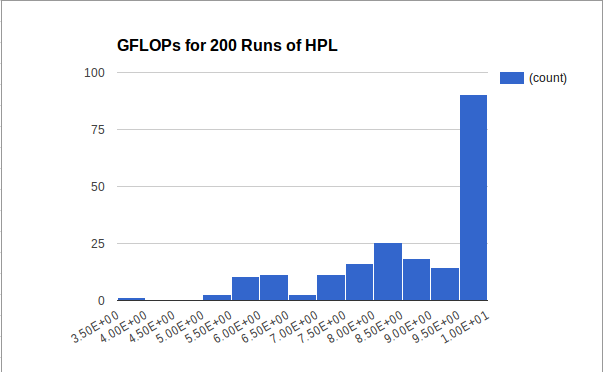
\includegraphics[width=0.42\paperwidth]{varsys.png}\\
	\end{column}
	\end{columns}
\end{frame}

\begin{frame}\frametitle{Why care about variability in simulations?
	A motivating example}
	\textbf{A toy parallel simulation optimization problem:}
	\begin{columns}
	\begin{column}{0.5\textwidth}
		\begin{itemize}
			\item Batches of sims requested by optimization
				algorithm -- evaluated in parallel
			\item Iteration tasks act as
				synchronization barriers
			\item Asynchronously
				distribute each batch of sims across 36
				cores
			\item Total CPU utilization (right)
				for 2 toy problems, with and w/o
				variability
		\end{itemize}
	\end{column}
	\begin{column}{0.5\textwidth}
		\includegraphics[width=0.42\paperwidth]{libe2_cpu_plt-eps-converted-to.pdf}
	\end{column}
	\end{columns}

	\par

	\medskip

	{\tiny
	Chang, Larson, Watson, and Lux.
	``Managing computationally expensive blackbox multiobjective
	optimization problems with libEnsemble,''
	in Proc. 2020 Spring Simulation Conference, article no.\ 31.\\}
\end{frame}

\begin{frame}{Statement of Problem}

	In this project, we are looking to
	\textbf{control throughput variability}\\

	\medskip

	\begin{itemize}
		\item Throughput variability must be controlled synergistically
			with expected throughput
		\item We treat this as a
			\textit{multiobjective optimization problem}:
			\begin{itemize}
				\item \textbf{maximize mean throughput}
				\item \textbf{minimize throughput std deviation}
			\end{itemize}
		\item As an example task, we use the
			High-Performance LINPACK Benchmark (HPLB) problem
			--- solve a dense linear system using
			massively parallel resources
			\begin{itemize}
				\item A sparse solver might
					be more representative of a
					sim workload; HPLB is a standard
					benchmark problem and often
					tuned
				\item The techniques used on HPLB are also
					relevant to most sparse solvers
			\end{itemize}
	\end{itemize}

\end{frame}

\section{Background and Methods}
\begin{frame}\frametitle{High-Performance LINPACK}
	\begin{itemize}
		\item HPLB throughputs are used to rank HPC systems on
			the HPC Top 500 list
		\item The standard solver for the HPLB is called \texttt{HPL}
		\item \texttt{HPL} has numerous algorithmic parameters that
			can be tuned
		\item Tuning \texttt{HPL} to achieve maximum throughput
			is encouraged before submitting to the Top 500
		\item {\bf We perform multiple runs of \texttt{HPL}
			at each configuration and consider the mean
			and standard deviation of the observed throughputs}
	\end{itemize}
\end{frame}

\begin{frame}\frametitle{Tuning HPL}
	We chose {\bf 6 integer-valued parameters} most relevant for tuning
	\texttt{HPL}

	\medskip

	All other parameters are fixed to recommended values

	\medskip

	There  are  over  $10^{11}$ possible combinations of these variables 

	\bigskip
\begin{center}
\begin{tabular}{c|cc}
    \textbf{Parameter} & \textbf{Lower Bound} & \textbf{Upper Bound} \\
    \hline
    $NB$ & $1$ & $256$\\
    $P$ & $1$ & $36$ \\
    $NBMIN$ & $1$ & $256$ \\
    $NDIVS$ & $2$ & $36$ \\
    $DEPTH$ & $0$ & $4$ \\
    $SN$ & $1$ & $256$ \\
\end{tabular}
\end{center}

\bigskip

	{\small Note: $P$ is the lead dimension of the $P\times Q$ processor
	grid --- Q is inferred based on $P$ and the total number of procs}
\end{frame}

\begin{frame}\frametitle{Multiobjective Optimization Problems}
	The multiobjective optimization problem (MOP):
	$$
		\min_{x\in{\cal X}} F(x) \qquad {\cal X} \subset \mathbb{R},
		\quad F : \mathbb{R}^d \rightarrow \mathbb{R}^p
	$$

	\smallskip

	{\it Pareto front} balances tradeoff between $p$ conflicting
	objectives:\\
	\begin{center}
		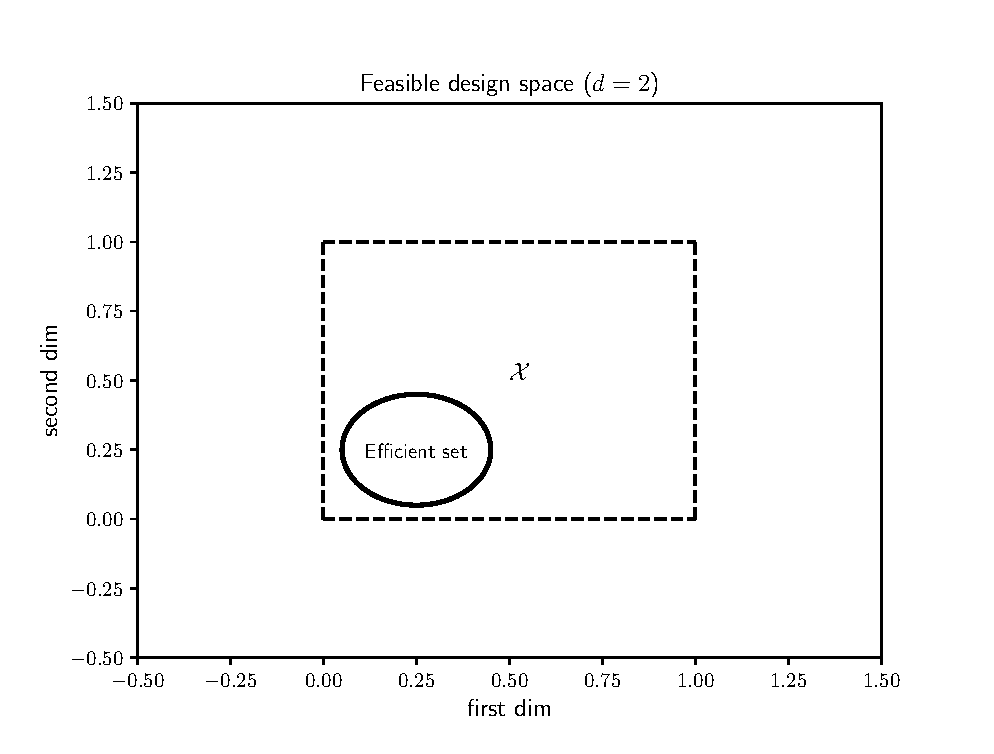
\includegraphics[width=0.42\textwidth]{feasible_design.eps}
		$\rightarrow$
		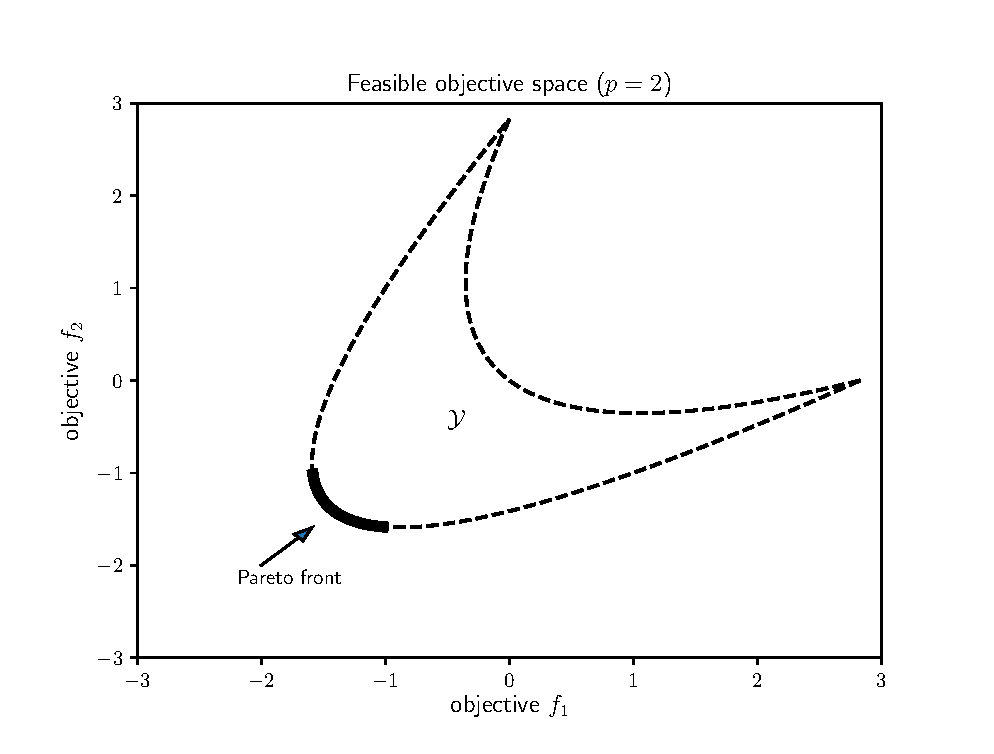
\includegraphics[width=0.42\textwidth]{convex_pareto.eps}
	\end{center}
\end{frame}

\begin{frame}\frametitle{VTMOP}
	\begin{itemize}
		\item \texttt{VTMOP} is a solver for computationally expensive
			blackbox MOPs developed at Virginia Tech in
			collaboration with Argonne
		\item Assumes ${\cal X}$ is a simply bounded set and $F$
			is a computationally expensive blackbox function
		\item Requires slight ``hacking'' to work with integer
			variables for tuning \texttt{HPL}
			\begin{itemize}
				\item Uses DIRECT and MADS to solve scalarized
					surrogate problems
				\item Must configure DIRECT and MADS to only
					sample on integer lattice
				\item Can be done by adjusting tolerances
					and ``binning''
				\item Further details in paper
			\end{itemize}
	\end{itemize}
\end{frame}

% Experiment 1
\section{Single-Node Experiment}

\begin{frame}\frametitle{The Single-Node Experiment}
	\begin{itemize}
		\item The single-node optimization of \texttt{HPL} takes
			place on an Intel Broadwell node of the HPC
			system \texttt{Bebop} at Argonne
		\item Each Broadwell node is a 36-core Intel Xeon E5-2695v4
			processor with 128 GB of DDR4 RAM
		\item The problem size is a $10,000$ variable linear system
		\item To calculate mean and variance, $40$ runs are done
			at each configuration
		\item In order to avoid wasted computation, if the estimated
			mean and variance after $5$ runs are worse than some
			threshold (see paper) the run is aborted and the
			low-fidelity approximation is returned
		\item \texttt{VTMOP} is given a budget of $2000$ evaluations
		\item The recommended configuration is provided for sanity
			check and to warm-start optimization
	\end{itemize}
\end{frame}

\begin{frame}\frametitle{Results}
	\begin{columns}
		\begin{column}{0.4\textwidth}
			24 approximately Pareto optimal solutions found:\\
			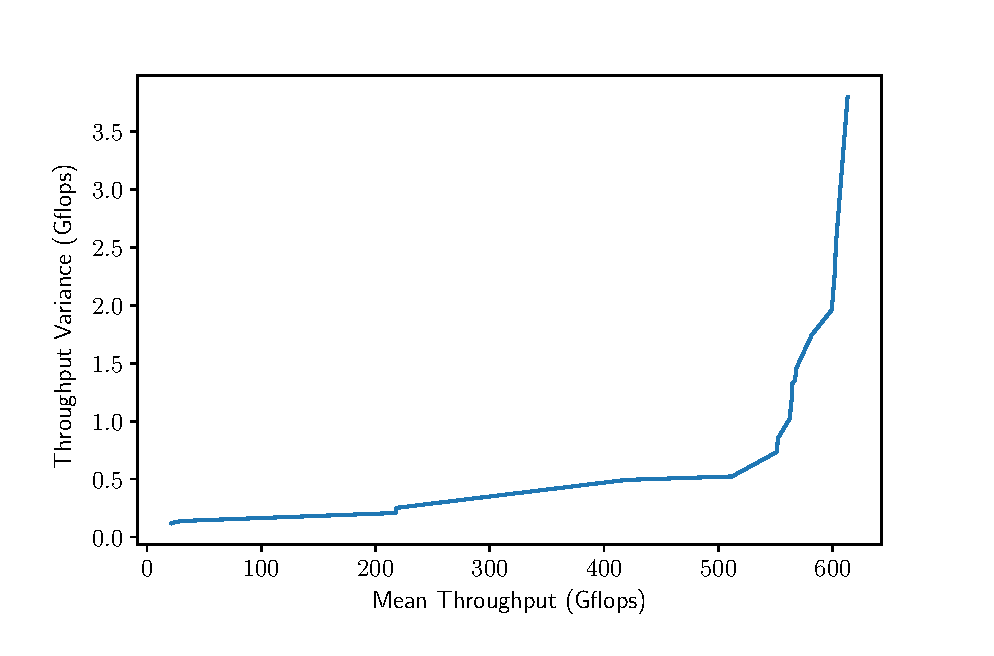
\includegraphics[width=1.1\textwidth]{hpl_n10k_pf.eps}

			\medskip

			{\bf Recommended setting is Pareto optimal},
			produces the max mean throughput:
			$\mathbb{E}[T(x)] = 613.04$,
			$\sqrt{Var(T(X))} = 3.8$
		\end{column}
		\begin{column}{0.6\textwidth}
			{\tiny
			\begin{tabular}{cc|cccccc}
    				$\mathbb{E}\left[T(x)\right]$
				& $\sqrt{Var(T(x))}$
				& $NB$ & $P$ & $NBMIN$ & $NDIVS$
				& $DEPTH$ & $SN$ \\
				\hline
  21.31  & 0.120 & 2   & 19 & 48  & 27 & 3 & 122 \\
  21.35  & 0.121 & 2   & 19 & 48  & 27 & 3 & 123 \\
  25.89  & 0.131 & 3   & 25 & 47  & 28 & 2 & 122 \\
  30.48  & 0.139 & 3   & 20 & 47  & 28 & 3 & 122 \\
  217.82 & 0.208 & 129 & 1  & 129 & 19 & 0 & 129 \\
  218.15 & 0.252 & 129 & 1  & 256 & 2  & 0 & 1   \\
  400.37 & 0.471 & 128 & 1  & 16  & 10 & 0 & 128 \\
  419.73 & 0.494 & 129 & 1  & 1   & 2  & 0 & 1   \\
  511.87 & 0.523 & 214 & 4  & 15  & 33 & 0 & 72  \\
  551.07 & 0.734 & 204 & 4  & 3   & 33 & 0 & 62  \\
  552.12 & 0.852 & 204 & 4  & 25  & 35 & 0 & 62  \\
  560.54 & 0.991 & 204 & 4  & 15  & 23 & 0 & 185 \\
  562.78 & 1.030 & 204 & 4  & 6   & 22 & 0 & 185 \\
  562.84 & 1.053 & 204 & 4  & 6   & 33 & 0 & 66  \\
  562.95 & 1.080 & 204 & 4  & 6   & 23 & 0 & 182 \\
  564.01 & 1.177 & 204 & 4  & 6   & 22 & 0 & 195 \\
  564.06 & 1.314 & 204 & 4  & 6   & 22 & 0 & 191 \\
  567.05 & 1.355 & 204 & 4  & 9   & 22 & 0 & 191 \\
  568.34 & 1.461 & 133 & 3  & 9   & 3  & 2 & 128 \\
  581.69 & 1.746 & 128 & 3  & 9   & 3  & 2 & 123 \\
  599.21 & 1.961 & 128 & 3  & 4   & 3  & 1 & 128 \\
  601.69 & 2.264 & 128 & 3  & 9   & 9  & 1 & 123 \\
  602.93 & 2.539 & 128 & 3  & 9   & 6  & 1 & 124 \\
  613.04 & 3.800 & 128 & 6  & 8   & 2  & 1 & 128 \\
			\end{tabular}}
		\end{column}
	\end{columns}
\end{frame}

% Experiment 2
\section{Multi-Node Experiment}

\begin{frame}\frametitle{The Multi-Node Experiment}
	\begin{itemize}
		\item Now using 4 nodes of \texttt{Bebop}
		\item Problem size increased to $20,000$ variables
		\item Only $s=30$ runs of \texttt{HPL} used for computing
			mean and variance
		\item Budget decreased to just $1000$ evaluations
		\item Because the budget was decreased, we eliminate the
			least important variable: fix $NB=128$
		\item The recommended configuration is given again
	\end{itemize}
\end{frame}

\begin{frame}\frametitle{Results}
	\begin{columns}
		\begin{column}{0.4\textwidth}
			24 approximately Pareto optimal solutions found:\\
			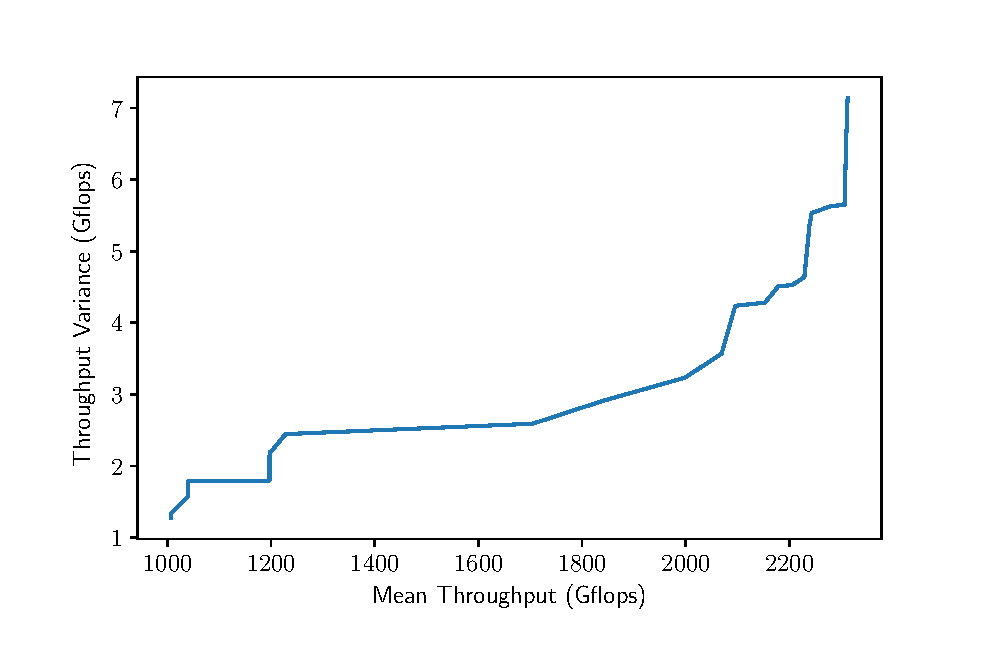
\includegraphics[width=1.1\textwidth]{hpl_n20k_pf.eps}\\

			\medskip

			Note the recommended settings produce the observations
			$\mathbb{E}\left[T(x)\right] = 2236.558$ and
			$\sqrt{Var(T(x))}=21.362$, {\bf not Pareto optimal}
		\end{column}
		\begin{column}{0.6\textwidth}
			{\tiny
			\begin{tabular}{cc|ccccc}
				$\mathbb{E}\left[T(x)\right]$
				& $\sqrt{Var(T(x))}$
				& $P$ & $NBMIN$ & $NDIVS$ &  $DEPTH$ & $SN$ \\
				\hline
  1007.1933 & 1.2741281 & 3 & 123 & 26 & 3 & 123 \\
  1007.4800 & 1.3432847 & 3 & 123 & 26 & 3 & 118 \\
  1040.2800 & 1.5831875 & 3 & 117 & 31 & 3 & 123 \\
  1040.3267 & 1.7903830 & 3 & 117 & 31 & 3 & 118 \\
  1196.7100 & 1.7968075 & 3 & 117 & 21 & 2 & 123 \\
  1196.7167 & 2.0589725 & 3 & 117 & 21 & 2 & 121 \\
  1197.0267 & 2.1971664 & 3 & 117 & 23 & 2 & 123 \\
  1199.9100 & 2.2000549 & 3 & 116 & 21 & 2 & 123 \\
  1227.7600 & 2.4454885 & 3 & 112 & 31 & 2 & 123 \\
  1704.5900 & 2.5906130 & 8 & 129 & 20 & 0 & 138 \\
  1840.7733 & 2.9114439 & 6 & 117 & 26 & 3 & 121 \\
  1998.3433 & 3.2330922 & 7 & 117 & 26 & 3 & 123 \\
  2069.1700 & 3.5682653 & 9 & 124 & 21 & 3 & 134 \\
  2095.6033 & 4.2372310 & 9 & 114 & 21 & 3 & 134 \\
  2153.0533 & 4.2825011 & 6 & 123 & 21 & 1 & 127 \\
  2178.2900 & 4.5079508 & 6 & 117 & 21 & 1 & 121 \\
  2205.2133 & 4.5274438 & 6 & 112 & 15 & 1 & 121 \\
  2228.8300 & 4.6360767 & 9 & 112 & 21 & 2 & 123 \\
  2238.9800 & 5.3728821 & 9 & 107 & 15 & 2 & 123 \\
  2243.0733 & 5.5329068 & 7 & 114 & 21 & 1 & 123 \\
  2281.7467 & 5.6351565 & 9 & 119 & 23 & 1 & 129 \\
  2306.3233 & 5.6427973 & 9 & 114 & 23 & 1 & 123 \\
  2309.9733 & 6.6279416 & 9 & 107 & 21 & 1 & 123 \\
  2312.3500 & 7.1394364 & 9 & 107 & 26 & 1 & 118 \\
			\end{tabular}}
		\end{column}
	\end{columns}
\end{frame}

% Conclusions

\section{Conclusion}

\begin{frame}\frametitle{Conclusions}
\begin{itemize}
	\item[{\color{red} \xmark}] I should tune \texttt{HPL} for variability
	\item[{\color{red} \xmark}] I should do a full multiobjective
		optimization of my kernels/solvers to figure out the best
		parameters for balancing variability and mean throughput
	\item[{\color{green} \cmark}] I should be mindful of
		\begin{itemize}
			\item[(1)] whether variability matters for my problem;
				and
			\item[(2)] how the parameters I choose effect
				variability in addition to mean throughput
		\end{itemize}
\end{itemize}
\end{frame}

\begin{frame}\frametitle{Acknowledgements}
{\small
This work was supported by the U.S.~Dept.\ of Energy (DOE) through the Exascale
Computing Project (17-SC-20-SC), a collaborative effort of two DOE
organizations, the Office of Science and the National Nuclear
Security Administration.

\medskip

This work was also supported by the Office of Science Graduate Student Research (SCGSR) program.
The SCGSR program is administered by the Oak Ridge Institute for Science and Education (ORISE),
which is managed by ORAU under contract number DE-SC0014664.
All opinions in this paper are the authors' and do not necessarily reflect the
policies and views of the DOE, ORAU, or ORISE.

\medskip

This work was also supported by the National Science Foundation under
Grant No. CNS-1838271 (the VarSys project: https://varsys.cs.vt.edu/).

\medskip

The authors gratefully acknowledge the computing resources provided on Bebop,
an HPC system operated by the Laboratory Computing Resource Center at
Argonne National Laboratory.}
\end{frame}

\end{document}
